\section{Introduction to Web Security}
In the recent $15$ years there was a strong increase in attacks that targeted multi-tier applications deployed on the Web. This increase follows in general two trends : it follows the trend of the growth of what we call Web $2.0$ applications, where the content is adapted to the specific needs of who is reading that and where web sites move from a situation in which they were mostly constituted by static content to a new reality where they represent full fledged applications. Naturally, protecting these kind of systems is way more complex than protecting a single standalone application on a pc, because simply there are way more levels of freedom that make these applications more dynamic, but on the other side make the job of security operators more complex. Notice that in this kind of scenario the critical components that needs to be protected are typically placed on the server side (DBMS server, authentication server, etc).

\subsection{OWASP}
This topic became so pervasive during the last $15$ years that a few initiative arose to try to provide a comprehensive view of the problem and suggesting meaningful and still simple practical solutions. Among the various projects, one of the most interesting is called \textbf{Open Web Application Security Project (OWASP)}. It provides some best practices to be adapted in order to make systems more secure. The basic principles suggested by OWASP for securing complex web application are the following :
\begin{itemize}
\item Apply \textbf{defence in depth} : it refers to the fact that the best practices linked to border-based defences are still good, as long as we define fine grained borders also within your premises. In other words, apply defense in depth means applying layered security both horizontally (working for different abstraction levels in our organization) and vertically for functions. This layered security allows us to create a lot more borders that we can control and enforce. Its main advantage is that if some adversary manage to overcome some of our defense measures at one of our borders, then there is quite a large probability that he will be able to gain an advantage point in our premises that is still not enough for him to reach its final intended goal. We should not rely on an unique defense.
\item Use a \textbf{positive security model} : typically it's depicted as a choice between two opposite sides using a negative security model or a positive security model. This latter one is historically the one that need be used and it's based on the usage of whitelist. The idea is that, whenever we apply this approach, we need to deny everything and then making exceptions by whitelisting them.
\item \textbf{Fail securily} : when a system for some reason fails, then is important to guarantee that it fails securily, i.e. errors are handled such that they do not creates security issues. From this point of view we can recognize two cases :
\begin{itemize}
\item \textbf{type 1 errors} : they are errors that happens during the processing of a security control. Obviously they should disallow the operation.
\item \textbf{type 2 errors} : they are errors that are exceptions in code that are not part of a security control, but given how this code is designed, they may affect the way a security control is performed.
\end{itemize}
\item Run with \textbf{least privileges} : with this approach we give to accounts the minimum amount of privilege that is necessary to perform a given operation. Of course, this privilege should last just for the time needed to perform such operation.
\item Avoid \textbf{security by obscurity} : it's a strategy where the idea is that if you want to encode things what you should keep secret is just the key used to encode, but then algorithm should be free, open and known to everyone, because it's not by hiding things that you will make those things secure.
\item Keep security \textbf{simple} : complexity could give us a false sense of security, but actually it's something that works against us. The more complex is a security system the easier it will be for it to contain errors, bugs, misconfiguration or bad design decisions.
\item \textbf{Detect} intrusions : it's fundamental to log security-relevant events and to ensure that they are periodically monitored, in order to act as soon as possible to limit and mitigate the intrusions impact.
\item \textbf{Don't trust infrastructure} : this means that understanding our infrastructure in details is fundamental to avoid errors and pitfalls that may give arise to incidents.
\item \textbf{Don't trust services} : typically most applications are constituted by a set of open source libraries that works in a coordinated manner, but we cannot expect that they are secure.
\item Establish \textbf{secure defaults} : we need to make sure that, even for people that are unaware of security pitfalls and threats, using our assets is something that can be in a secure fashion. We may possibly give the opportunity to make informed choices how secure is the usage of our assets and resources.
\end{itemize}
This practices works for a wide variety of potential risks on server side, client side, but also for ones that comes from the network.

\subsubsection{Server side risks}
They are typically the most effective ones and they are related to different objectives that adversary may have when they plan how to attack the servers we are running. Their goals are typically the following : \textbf{data stealing} (i.e. data breaches), \textbf{remote command execution} where the attacker is trying to deploy and execute on the target machine, code that is written by himself for various purposes, collecting further data for setting up more complex intrusions or attack the machine through a DOS to interrupt the services provided by such machine. We are dealing with the security of applications that offers services to end users, and it's important that these services are offered in a safe way such that the users will be able to access functionalities offered by services as they have been designed by the system designers. An attacker to subvert the functioning of the server is to modify the application itself either to hide behavior that not directly visible to the users like steal their information or possibly to push the users to do some actions that would never do in a normal scenario. For this reason the Web server that run the application plays a fundamental role. In particular, it's very important that their configuration is appropriately managed by system administrator to make sure that content and applications are executed in a safe environment. From this point of view there are few elements that we need to take into account :
\begin{itemize}
\item \textbf{document root} : it's the folder where the web server will look for content to be served against users requests. Typically inside this folder we will find documents and files that represent the starting point to serve the content towards the users. Clearly the document root is another delicate point in the configuration, since its content needs to be reachable from users with privileges such that to avoid that they can possibly execute code that they provide inside this directory.
\item \textbf{server root} : it's the directory where the files and executables needed to correctly execute the web server are actually located. It typically contains few scripts, logs and configuration files. It's fundamental to protect this directory, since for example the logs files may contain sensitive information such as session key, and an attacker may try to steal it in order to replicate a valid session. Furthermore, this directory has a lot of space and subdirectory that can be accessed with different level of rights in order to correctly execute the server. However, an attacker may leverage such space to inject its own executable and make it run when the server starts, and he could leverage it for example to receive commands from a remote server. 
\end{itemize}

Most of these problems boils down setting up these directories with the correct file permissions wrt the configuration of the web server. In particular, we need to take into account that document root will contains mainly documents that just need to be read and that server root will contains files that needs to be execute or documents that shouldn't be accessible from normal users. A common approach used to secure directory and user access rights is by defining specific user name and group for managing the access rights to these two directories (e.g. www \& wwwgroup). Typically, the server root will be the home directory of www user. Instead, the wwwgroup is used to make sure content editors will be able to access directories with the correct rights to write new documents inside the document root and its subfolders. For the server root typically only the www user should have read/write/execute privileges everywhere within such folder and its subfolders. Users part of the wwwgroup may have read and execute access everywhere, but write permissions only on content that needs to be updated. Notice that the web server should run with a user called \textit{nobody}, which has minimal access rights on the target system. This means that clients accessing the web server will have exactly those rights. For this reason, it's important that the document root will give permissions for reading and executing to other users different from www user and the ones in wwwgroup. In some cases, we may want to implement through the web server selective access to the content of the document root depending on the browser's IP or authentication. However giving permissions to all users to be able to read those documents is not a good idea, because all local users will be allowed to access that content. In this case, we may possibly reconfigure the server to run with a different user from \textit{nobody}, provided to that user minimal privileges and belongs to the wwwgroup. In that case, we need to make sure that such group has a restricted access with write rights to specific sections where we know that the users will not be able to do any damage. If for some reason, the web server runs with a user different from \textit{nobody}, we need to make sure that no log directory is writable for that user id, otherwise it may possibly be used by an attacker to write code to be execute or to gain access to protected data like the passwd file, by simply creating a symbolic link within the log directory and then read that symbolic link. In the typical scenario, the web server is started as a daemon with user id root, and this is needed to allow the server to stay listening on reserved port such as $80$ or $443$, and to write log files in a protected place. Naturally, if someone connects to the web server, this latter accept the connection and spawn a new child process that will be executed with limited privileges (typically with user \textit{nobody}). This is a robust scenario because it allows the web server to have full control of the machine for correctly serving the incoming requests and make sure that such requests can be handled by low privileges processes such that if any of these processes is subverted the impact of the compromisation is as small as possible. If we allow to run the child processes with root privileges, then everything can be accessed by the users and possibly the attacker can use the vulnerabilities in the code executed by the web server to make damage like only an administrator can possibly do. Another scenario, is where not even the parent process has root privileges. However, in such case the web server won't be able to open port $80$ and neither other well-known port.\\\\Some optional services that may be offered by web server and that represent another source of concern of security risks. In particular, most web servers includes the following services :
\begin{itemize}
\item \textbf{Directory listing} : it's a service that allows the users to get a directory listing. This is a strong problem, because we may end up stuff in document root that represent backup files, temporary directories and files. Notice that just disabling this service, doesn't prevent attackers from accessing these files.
\item \textbf{Symbolic link following} : it's a service that allows requests to follow symbolic link. It represent a possible security risk, because if in the document root is present a symbolic link to an external file, then a client that request to access to such link will read the content of the linked file. A possible solution is to use some configuration opportunities provided by the web service (e.g. aliases) to extend the document tree beyond the limits of the document root. In this way the configuration is more explicit wrt a symbolic link.
\item \textbf{Server side include} : it's a simple way to include in static content some small snippets of dynamic data, that was provided by incorporating an external file or including in the html static content the result of the execution of an external process. In particular, among the various server side include directive there was the \textit{exec} directive, that allows the execution of external scripts or shell commands, took the outcome and include it in the html file before serving it to the client. This is a common security risk because it allows, if not appropriately controlled, to make the attacker run more or less any potential script in the system and serve whichever content he wants. Today most of the functionalities that were formerly proposed through server side include are implemented by more complex full fledged server side scripting techniques based on various languages such as PHP, Python, etc.
\item \textbf{User-maintained dirs} : it's a service that allows users to automatically add to document root personal portions of file system. This is potentially a strong breach in security, because in the end server administrators typically are not able to fully control what users actually do.
\end{itemize}
There are also some cases where content creator are given the possibility to access some sections of the document root through another service like a ftp server, that was used to update the content of the web server. The problem is that now we need to guarantee a coherent configuration of both servers in order to avoid potential vulnerabilities to arise from their possible connections. An approach that is sometimes used to enforce a bit more security on web servers is to use \textit{chroot} command, which creates a limited execution environment with root the provided path. The problem with this kind of approach is that processes will only see things that are visible through the new root. In this environment we can avoid to include any interpreters or sensitive data that can potentially be used by an attacker to execute code or steal information. Another important approach that is used to secure the environment that is around the web server, is to isolate the web server wrt other potentially sensitive assets like hosts and networks that need to be better protected. This approach stems from the idea that the web server is something that needs to be accessed by anonymous users. While other parts of our networks don't have this kind of requirement. This approach is realized in such a way that, even if the web server is compromised, the attacker will not be able to get into the entire network. Typically the server is placed in an isolated network area called \textbf{Demilitarized zone (DMZ)}, which controls the access from the internal network to the web server, and forbids the access from the web server to the internal network. The implementation of this kind of network segmentation is done using an appropriate use of the firewall, which may give arise to the following approaches :
\begin{itemize}
\item \textbf{Dual homed host} : in this case the firewall is equipped with two independent network interfaces, one is attested on the Internet and the other one is attested on private network, the routing between two interfaces is disabled by default, and packets are allowed to flow between the Internet and the private network only by passing through an appropriate application that perform in general application level filtering. In this case we would place the web server between the dual homed host and the Internet, but the problem is that this kind of configuration is not flexible, because any exception requires an appropriate rule to be written at application level within the dual homed host to allow packet flows and with large networks this hardly scale.
\item \textbf{Screened host} : this approach is based on a router called \textbf{screening router}, which is configured to block any connection from the Internet to a protected network, but any of these connection attempts is redirected to a special host called \textbf{bastion host}. It's the only host present in the protected network that allows to access and receive connections from the Internet, and in practice it acts like a proxy wrt any connection that goes from the Internet to the protected network and viceversa. Clearly, the bastion host needs to be strongly protected (hardened setup). It's often realized through secure operating system that are standard operating system configured to offer as less services as possible such that they will not be exploitable by attackers. Every activity happening on the bastion host is immediately logged and placed on a secure log service such to be continuously monitored for possible traces of incidents.
\end{itemize}
Another important aspect to take into account while protecting server is to continuously monitor what is happening in that server. The server typically exports information in a  detailed log that contains all information about which kind of actions are performed. The idea is that if the server is compromised, the log can be modified by the attacker, in order to hide its activities. In this case it makes sense to equip the server with a host-based intrusion detection system, which is a software that runs together side by side with the server on the same host, and continuously check and analyze what the server is doing. They are able to intercept some suspicious activity and in such case they may possible raise an alarm or take some remediation action such as terminating that specific process and so on so forth.

\subsubsection{Client side risks}
From the client side, most of the risks are related to the browser. They are a good target for attackers because they may possibly be used to run the user code to call whichever effect may be the interest of the attacker such as browser crash, damage the user system, etc. In particular, the violation of end user data is a compelling scenario, since these data can be used later to perform identity theft attacks. In general, the attacker may use the vulnerabilities present in the user browser to attack the user itself by compromising a system as soon as a system visit the website, possibly delivering on the machine code that represent malicious software like trojans or spywares. An example of trojan is the following : we visit a website which download and execute on the web browser some client side code that exploit a local vulnerability. An example of spyware is the following : it's a software that sell itself for performing some legal action on the system, but they are written in a tricky and unclear way in such a way to push the user to accept the proposed conditions, making him subject to some type of legal data stealing from its machine. Today there is a security policy that is enforced by all browsers called \textbf{Same origin}. The idea of such policy is the following : if you visit a website and you exchange some data with that website, another website cannot access that data. The term origin is defined using the domain name, application layer protocol and port number of html document running the script. Two resources are considered to be of the same origin if and only if all these values are exactly the same. Why this policy is so important ? Because it allows the browser to implement easily a strong security policy that somewhat create some clear and unavoidable barriers between distinct applications and avoid these applications to inadvertently exchange information. 
\paragraph{Cookies} They are simple pieces of information that a website can store on a visitor web browser. It's a way to overcome the main limitation of http protocol, which is the fact that it's a stateless protocol, i.e. it doesn't maintain any conversational support. For this reason the standard builders decided to introduce the cookies as a tool that can be used for several distinct things, and among these things is to implement a simple mechanism to track user sessions. The idea is that every time a web browser request a web page, the web server will provide the content that has been requested, but it may also include some headers that includes cookies. These cookies are simply small bits of information. Typically to track session the web server will include a session ID (a pseudorandom number which is with high probability unique and that will uniquely represent that user every time the user interacts that web server during that session).
\begin{center}
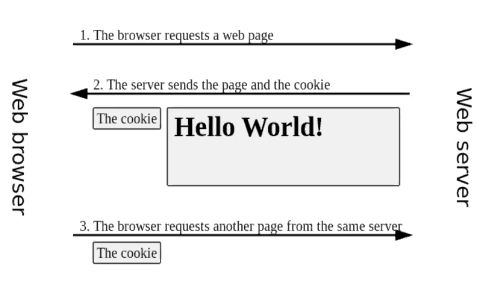
\includegraphics[scale=0.5]{./images/cookies_schema.png}
\end{center}
Once the cookies are stored in the web browser, every time the browser will make a new request to the web server, it will send together with the request the cookies. On the web browser, cookies are stored locally in a dedicated storage and it will make sure that they are send back to the web server only when the user is visiting the web server for which that specific cookies has been designed. In particular, each cookie will contain a few components such as name and value (mandatory), plus other optional components such as expiry, path, domain and need for a secure connection. Typically, we can find two kinds of cookies :
\begin{itemize}
\item \textbf{session cookies} : they are removed when the browser quits (they do not have an expiry date)
\item \textbf{persistent cookies} : they are cookies that has an expiry date which remains on the client until such date. Typically, they are not kept in memory, but they are also saved somewhere on disk. Their typical usage is for example to automatically authenticate again the user as long as he tries to log in in a near future.
\end{itemize}
Another interesting way to look at cookies is by differentiating between :
\begin{itemize}
\item \textbf{first-party cookies} : they are provided by a website that we target directly by making a request through our web browser. 
\item \textbf{third-party cookies} : they are injected by other websites that we don't have directly visited or we didn't do that explicitly. This may happen for example if we visit a website $A$, which provides the content we are requesting and possibly also includes some first party cookies. Then our browser analyzed the content that has been received by $A$ and while rendering the web page it encounters an element in the page that requires further content be fetched by another website $B$. In order to do that the browser will open a new connection toward domain $B$ and through http request ask domain $B$ to provide the resource that is needed to correct render the page. While providing that resource website $B$ has the opportunity to send back to the browser a cookie (this is consider a third-party cookie). This is typically a trick that is widely used by marketing companies to implement large scale of tracking of users preferences. In fact, the tracking is obtained by embedding in a web page an advertisement that will keep track for example of how frequently the user will visit such web page. However, there is still a problem, because the same origin policy doesn't allow website $A$ to exchange information with website $B$. In the standard scenario the website $A$ will make a request to website $B$, but will not include the cookie that are stored by it, because this will violate the same origin policy. What $B$ can possibly do, is to store on our browser information about our identity from its standpoint. The two identities on $A$ and $B$ are not obviously linked. However these two identities needs to be linked in some way in order to allow an exchange of tracking information between $A$ and $B$ for a particular user. How can they do that without violating the same origin policy ? They can use the so called \textbf{cookie syncing} approach. The idea is the following : when we ask $A$ to provide a content at the beginning of a session and provide our user ID, $A$ before serving us the content will provide us with a redirect http response that will point us to website $B$. In this request $A$ will include both its ID and our user ID as its known by $A$. Our web browser will bring us to $B$ sending these information plus the cookie for such website. At this point $B$ will match our local user ID with our remote user ID on website $A$. Now, for $B$ is enough to redirect us again to $A$ with an information that will tell website $A$, "ok, i've synched the ID, you can proceed with serving the original content". How much can we protect ourselves from this kind of information leakage ? The most extreme solution is to use an ad-hoc solution that completely anonymize our usage of the web (e.g. TOR). Another approach is at least protect our point of access to the web by using a VPN. The usage of cookies for tracking user preferences is more and more endangered on one side by technical advancements like those introduced in the browsers and on the other side by regulators that tend to limit the freedom of tracking services to do whatever they want to profile users. However companies continuously look for new solutions to overcome these limitations. An example are the \textbf{super cookies}, which are information still stored in our computer by non-traditional methods. They are persistent, but the fact that they are not real cookies, they tend to be ignored by both regulations and technical means to get rid of them.
\end{itemize}

The risks coming from the network are linked mainly to actions that the attackers may perform by interposing itself between the two endpoints that are communicating. The basic attack is linked to \textbf{eavesdropping} to capture data that are exchanged between the browser and the server, and possibly make use of these information. 

\subsection{HTTP authentication}
For accessing a lot of online services we need to authenticate ourselves. We have a physical identity, but then we act in a virtual world using a digital identity (a representation of ourselves in the digital world). When we asked to authenticate by a service, the service will challenge us to prove the fact that our physical identity can be represented by a specific digital identity while using that service. Authenticating means proving that there is a match between our physical identity as user that is accessing that service and the digital identity that we will use for accessing that service. There are several ways to authenticate users. We will start talking about \textbf{HTTP authentication}. It's a protocol performed by landing on a web page that requires authentication, where the web server will fires up the request for authentication and the browser will answer asking us to provide a digital identity in the form of a username and password that confirms the link between that digital identity and ourselves. The HTTP authentication is typically configured on the server side by configuring in the proper way the web server. It implements two different challenge-response protocols :
\begin{itemize}
\item \textbf{Basic authentication} : assume that we perform a request for a resource on a web server and the server is configured in such a way to require authentication in order to access that resource including in the response header the WWW-Authenticate header that will include at least the form of authentication required plus realm=string. The realm concept is used to contextualize the authentication to a specific security realm on both the client and server side. When the client browser receives the $401$ error message since the client didn't performed any authentication yet, it will show to the user the classic popup asking for username and password. The username and password will be send back by the client towards the server replicating again the same request, but adding the Authorization header that will contains the type of authentication used plus a string. This string contains an encoded version of the username and password (Base64 encoding of username:password string). When receiving this request with the header, the server will take the content of the username and password from such string, checks the credentials locally, and if everything is ok, it will return the status code $200$ and serves the request, otherwise it will send back the $403$ error code. We want to underline that this schema doesn't use any encryption method, so it's very easy to decode such string in order to retrieve the user credentials. 
\item \textbf{Digest authentication} : It's an authentication method slightly more secure than basic authentication. In this case, the server challenges the client using a nonce (together with www-Authentication and realm header). Then the browser will again ask the user to provide username and password, and it will the information using again Authenticate header, with the username in plaintext, the nonce received from the server, the realm, the uri of the service that needs to be accessed, a response (which is a cryptographically hashed version of the username and password) and the algorithm used to compute the response. The client to compute the response uses a predefined a cryptographically secure hashing function such as SHA256, and then simply first applies the hash to the string username:realm:password, then it applies the hash to method:digestURI and finally will it will hash the string constituted by the first hash computed, followed by :nonce:, and the second hash computed. The server replicates the same approach and then will check coherence of the calculated hash with the response that was sent by the client.
\end{itemize}

Another type of authentication is the \textbf{form-based authentication}, which is a simple way include all those authentication methods that rely on the user sending credentials through some kind of html form. It basic idea is that the user is redirected to a specific web page on the web application that he's using. This web page provides the basic form where it request the user to provide its credentials. Naturally, the requests to this page needs to be protected through TLS. So the user filling the fields with the username and password, click the button to submit the credentials that are sent through the secure channel towards the web server, which it will validates the user identity. Exactly like the previous methods, it's designed to overcome overcome the limitations imposed by the stateless nature of HTTP. By asking user to authenticate, the web application fulfill two different goals at the same time : on one side it creates a persistent session for the user, and on the other side it associate this session to a specific virtual identity. What the server typically does upon authenticating the server, it sets through a cookie a session ID for the authenticated user. This session ID needs to be protected, because it represents the authenticated user for the duration of its usage of the website. So, from this standpoint, the session ID represents the identity of a logged in user. This means that if someone is able to sniff and steal that session ID, he may possibly to impersonate the user by sending new requests and independent from the ones of the real user, sending also the session ID. In this way the attacker is able to fully impersonate the user, unless the server implements some techniques to avoid this kind of attack. This attack goes under the name of \textbf{session hijacking} or \textbf{cookie hijacking}. So keeping the client-server channel secure by encrypting it by TLS is a fundamental requirement to implement form-based authentication and the subsequent secure session IDs secured through out the whole session. However, this is not the only way session hijacking can be performed. Indeed, if the attacker knows that the client-server channel is encrypted through TLS, he will look for alternative solutions to steal the session ID (attacking the server or the client). The security of the browser is typically linked to two aspects that are tightly coupled with the user that is actually using that browser (browser bad configuration or when the user give the permissions to the attacker to be attacked without understanding that). Fairly more frequent are attacks that target the server side. This kind of attacks typically target the front-end of the web application. They may have different purposes : target the web application to subvert the functioning of the web application, to steal data from the web application, attack specific users. Now, we want to talk about \textbf{unvalidated input} which is a typical software design flaw that give rise to different vulnerabilities that can be exploited with different kinds of attacks.

\paragraph{Unvalidated input} Typically all web applications rely on the standard HTTP request-response protocol to provide their functionalities. If the client is an attacker he may try to subvert the application functioning by tampering with the content of the data streams exchanged between clients and server. The server will take the data whenever it comes from and will possibly interpret them, or to use them to implements some functionalities. Now, if the web application blindly relies on the trust that it has towards its users, bad things may happen. Any data considered by the web application from the user input to be used for any reason, these data needs to be validated before its usage. Unvalidated input from the user may possibly give rise to different kinds of attacks such as XSS, injection flaws and buffer overflow. Validating the input means implementing some functionalities that checks if the input provided by the user is fully compliant with the input that is expected by the application. There are several problems in implementing user input validation : client side or server side input validation ? However, the first approach is completely useless against a dedicated attacker, because he will simply skip them. So, the common case is that we should always implement input validation on server side. In order to proceed with input validation we need to use what is called \textit{positive input validation}. It means that we as software developed should explicitly define the format and limits of the input that we expect. For example we can specify the minimum and maximum input length, the allowed character set, whether null is allowed, specific patterns and so on so forth. A kind of buffer overflow attack that comes from unvalidated input is the \textbf{Heartbleed attack} (for more information about that see \href{https://www.vox.com/2014/6/19/18076318/heartbleed}{here}). 

\subsubsection{XSS}
Another common kind of attack that comes from unvalidated input is \textbf{cross site scripting (XSS)}. XSS is a kind of attack that is strictly related to web applications. The typical case of a XSS attack is the following : there is a web application somewhere, that acquires data from a non-secure source (i.e. user input). The acquired data are sent to other users : they are the target of the attack. Once these users visit the compromised web application, they will receive data from the web application that contains input provided by malicious users. If this input contains client side code, this code is executed on the user browser. 
\begin{center}
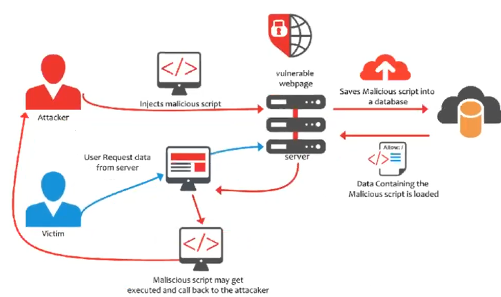
\includegraphics[scale=0.4]{./images/xss_scenario.png}
\end{center}
An interesting web site to understand which are the most common attacks against web applications is \textbf{OWASP Top 10}. In particular, the information for each attack are divided in three aspects :
\begin{itemize}
\item \textbf{Attack vectors} : this section contains information about how an adversary may possibly implement the attack
\item \textbf{Security weakness} : it contains which kind of weaknesses enable this kind of attack and how we can possibly get rid of such weaknesses
\item \textbf{Impacts} : it contains information about the potential impact of this kind of attack.
\end{itemize}
A typical way to perform a XSS attack is to embed some user input into a snippet of html code (e.g. inject a script in the $\langle a \rangle$ tag). In particular, there are three common variants of XSS attacks :
\begin{itemize}
\item \textbf{Stored} : it's a situation where the attack script is already stored somewhere on the website. The attacker uses a vulnerability present in the website, for example a form that doesn't correctly validate the input, to store in a database a malicious script. Then the content of the database is used to serve content to other users, and these users may end up running the malicious script.
\item \textbf{Reflected} : it's a situation in which the user is pushed by the attacker in making a request to the vulnerable web server, that will send back the attack to the user itself. So the source code of the script is not stored in the server, but is the attacker that through some way (e.g. phishing email) push the user in sending the attack script to the server, and the server reflects back the attack script to the user, that is then compromised.
\item \textbf{DOM-based} : We may have a vulnerable web page that includes a script that is provided by the web application itself. Some of these scripts may do some use of information that are provided by the user itself. If the input is not appropriately validated, then it can be used to perform a XSS attack. It's called DOM-based attack because the attack is not directly served by the vulnerable web application, but the attack is actually served by the user browser itself that renders the code containing the attack only at the end of the execution of some legit script provided by the web application. A difference with the previous approaches is that the vulnerability is executed on the browser, not anymore on the server.
\end{itemize}

\subsubsection{CSRF}
Another kind of attack we want to talk about is \textbf{Cross Site Request Forgery (CSRF)}. It's similar to XSS attacks, the real difference is that we are not using scripts anymore, but rather we are targeting directly the web application using the user as a vector. The idea of CSRF is that the attacks works on the basis of a simple assumption : the web application is trusting whatever an authenticated user do. The problem is that the attacker with CSRF can push the user to send a request towards the vulnerable web application, without obviously the user being aware of that. The attacker proceeds as follows :
\begin{enumerate}
\item First of all the attacker observes how the users interact with the target web application. In particular, he may try to focus its attention on how the users provide data to the web application.
\item Next the attacker builds a fake request that mimics a valid user request. The only problem is that the attacker can't be considered trusted from the web application without a valid session ID.
\item To proceed the attacker lures an authenticated user to visit a website where he has included the form to be submitted (hidden wrt the user). Once the user visit the web page the request will start automatically. Thus, the data submission should be triggered silently and automatically as soon as the user visit that malicious web page.
\end{enumerate}
\begin{center}
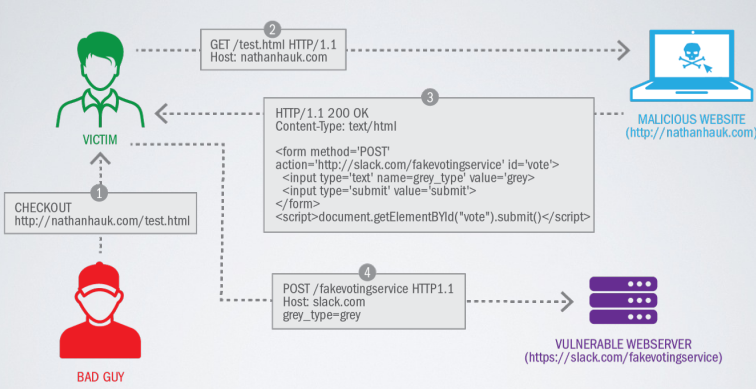
\includegraphics[scale=0.5]{./images/csrf_scenario.png}
\end{center}
How does the attacker perform a CSRF attack in practice ? Typically he needs to use a proxy to intercept a non malicious request, in order to understand how the request is performed, because he need to recreate it carefully. Then he setup the malicious web page that contains the CSRF attack with the hidden form and javascript to perform auto submit. Finally, the attacker send the phishing email to the user. The problem is that the target web application blindly trust the requests coming from authenticated users. The problem here is that the web server handles the request even if it's not actually following another request where the user asked the application to provide the form. The solution to this problem is to make sure that all form submissions requires some sort of random token to be submitted every time called \textbf{CSRF token}. This token is defined for each user session and be unique, secret and unpredictable. So every time the web application send a form to the user, it will include the CSRF token in the form as a hidden field such that every time the user click submit on the form, the value of the CSRF will return back to the web application and it will be able to check if the content of the token included in the form submission is equal to the token that was defined for that session. If the two are the same token, then it's a request that is coming as a consequence of serving a form to the user. Otherwise it's a potentially CSRF attack.

\subsubsection{SQL injection}
Injection flaws is a class of vulnerability that allows an attacker to circumvent the functionalities provided by the application and make the application execute code that was not in the original design of the application itself. This is the reason why they're called injection flaws, because they allows the attacker to inject its own code in the application and execute the code in the application context. The most common injection attack is called \textbf{SQL-injection}, which allows an attacker to inject code in the application in places that actually accepts user input, that will be executed by the interpreter behind the web application itself. In SQL injection attack typically we have that the application on the server makes use of a database back-end to store and retrieve data that is then presented to the user. How does SQL injection works ? The idea is that instead of providing the expected user input to the web application, we provide SQL code to be injected. In fact, the typical scenario, will dynamically creates a SQL query using some data provided externally that can possibly be altered by the attacker, without good validation of such data. Naturally, the target of this attack is always the server that serves the application and the attacker goal is to perform operations that are typically not directly authorized. An important aspect is the fact that if we just consider the case where the attacker wants to inspect and extract data from the database, the problem is that the attacker is limited by how the output of the query is used to craft the interface that is then returned through the web response. In this case the attacker needs to use a different technique that is called \textbf{blind SQL injection}. In blind SQL injection the attacker doesn't see directly the result of the query, the only thing that he can see is a binary result (e.g. an error occurred or not). In this case the attacker may ask to the database true/false questions in order to extract 1 bit of information at a time. In order to be robust against SQL injection we need for sure to validate in a proper way the user input, then we can also use additional options such as \textbf{parameterized queries} or \textbf{stored procedures}. The former are predetermined queries with placeholders that are provided by the runtime environment where the application is actually running. The parameters provided by the user input are used to provide values to those placeholders. The latter are subroutines that are provided by the DBMS itself, which can validate input at server side.

\subsubsection{Broken authentication}
Authentication being a critical functionality of a web application is typically subject to several kinds of attacks. In particular, it may present vulnerabilities that if correctly exploited by an attacker may allows the attacker to impact the security of the application. Broken authentication methods are mainly based on problems linked to how password-based authentication is performed and how session security tokens are handled. When dealing with the authentication and the usage of reserved functionalities from users, typically we need to take into account two aspects : the authentication (link between physical and digital identity) and the second one is how do we authorize a specific user represented by a given digital identity to perform or deny the access to some specific functionalities. Password-based authentication has some well known and strong limitations that are mainly related to how password are chosen and managed by the users and website. In particular, attacks to such schema may be related to several aspects of password management. Notice that whatever we do for implementing a correct password management at the server side, the weakness can be on the user side, because most users continue to choose bad password for their digital identities. Predictable passwords are bad because they are an easy target for dictionary-based attacks, reused passwords are even worse, because allows the attacker to perform the so called \textbf{credential stuffing attack}, where they have large databases of real password and then try them again and again on real accounts to check if anyone decided to reuse its own password. There are some best practices in how to push users to choose in the right way their passwords. The first practice is pushing people use password managers. Password managers as long as they are used with a local database of passwords, are good solutions for forcing people to use complex passwords because the passwords are generated randomly by the password manager and use different passwords for different services, since the password manager store all passwords for all services and the user needs to remember one single complex password to access the password wallet. The other approach that should be used is the usage of two factor authentication. Using two factor authentication means we challenge the user for at least two authentication methods. Regarding password management at server side we shouldn't store
\begin{itemize}
\item passwords as plaintext, because they are easily captured at server compromising
\item encrypted password, because if the server is compromised it's likely that the encryption key is also compromised
\item secrets (e.g. password digest) deriving from passwords, because digest of dictionary words are easily attacked.
\end{itemize} 
Sessions are subject to attacks through several approaches such as XSS. In fact, in a reflected XSS scenario we trick the user in sending appropriately crafted javascript code to the web application that reflects it back and make the user browser contact an external service controlled by the attacker and pass to this service information about the session ID. The session ID at that point is linked to an authenticated user and can possibly be used by the attacker to impersonate the user in the vulnerable application. Notice that we can mitigate it in several ways : by setting up the session cookie as a \textit{HttpOnly} cookie the browser will avoid from sending that data together with the other cookie towards the adversary controlled web site. Another approach is to make sure that, during a session, the session ID is linked to a specific IP from which the user was contacting the server. Another kind of attack related to sessions that stems from a wrong implementation of session management is the so called \textbf{session fixation} attack. The basic idea is that the vulnerable web site accepts any session identifier. The web application should be designed in a way that it will accept client requests bringing only a session ID that have been issued by the application itself and that it's not expired. This check needs to be done for each single client request. Otherwise the attacker can send an email to the victim, tricking him in contacting the vulnerable web application with a request that already contains a session ID. In this case, if the victim trust the attacker, the user will be challenged for authentication on the vulnerable web application, he will issue its correct credentials and at this point the session ID that have been crafted by the attacker will be associated to a valid identity. To mitigate this kind of attack, the server needs to check that each single session ID that is created, is stored somewhere for its entire lifetime and during its lifetime it can be only associated to a specific user and after its expiry date the session ID should be delete. Furthermore, when a user perform logs out from the web application its session ID should be delete. In such a way, the attacker is not able to reuse session IDs associated to previously logged in users. Another attack is called \textbf{session sidejacking}. It's based on the idea that the attacker may possibly setup an attack where he tries to sniff the content of requests between the user and web application. Some sites use TLS encryption for login pages to prevent attackers from seeing the password, but do not use encryption at all for the rest of the site, once the user is authenticated. However, the attacker may sniff the network traffic to intercept all the data that is submitted to the server, including the session cookie. This is one of the reason why today most applications tends to switch to a new model where everything is always served through secured channels. Notice that beside the usage of secure channels, session hijacking attacks can still happen if the user machine has been compromised through a malware, because in that case the malware may possibly tamper the web browser stealing the session ID from the browser memory space and sending it to the attacker blindly for the user.

\subsection{CSP for mitigating XSS}
In order to mitigate XSS, we say that this is a consequence of the fact that there is a vulnerability on the server side, because typically user provided content is not correctly validated. Can we do something on the client side ? Yes, we can use CSP to mitigate various types of attacks, including XSS. In practice, CSP is made up by a HTTP response header that instruct the browser on how to make use of the scripts and content that are loaded starting from the web page that is served. In particular, this will limit the kind and origin of scripts that can loaded. CSP is based on the idea that server administrators can through it reduce or possibly eliminate all the vectors through which XSS attacks are executed. In practice, the server provides all content to client that perform the request including a content security policy through which a policy is defined (i.e. \textit{Content-Security-Policy : policy}). In the policy what the administrators does is to specify a set of directives. Typically every policy should include a \textit{default-src} token that identifies the default source that is accepted for content that should be loaded together with the web page (e.g. the \textit{self} value means that, by default, content can be freely loaded by the browser from the domain itself from which the web page was loaded). We can also specify directives for handling different kind of resources such as \textit{img-src} for source of images, \textit{media-src} for source of medias and \textit{script-src} for source of scripts, etc. This is effective because it reduces the options the attacker has to include in a target web page some external content. In addition to whitelisting domains, the policy can also provide two other way to specify trusted resources :
\begin{itemize}
\item The CSP directive can specify a nonce and the same value must be used in the tag that loads a script. If these value doesn't match then the script will not be executed.
\item The CSP directive can specify a hash of the contents of the trusted script. If the hash of the actual script doesn't match the value specified in the directive, then the script will not be executed.
\end{itemize}

\subsection{Access control attacks}
In general access control is a system implementing a methodology that enables some authority to control how users can access specific areas and resources that are made available by an application. In particular, through access control systems we can decide which specific user is allowed to access some specific resource. Notice that access control mechanisms are typically a critical defense mechanism for any applications. When an access control mechanism is defective, typically the attacker can take control of the full application. They are typically tight to the specific applications that are complex to implement and they are often a source of errors. We usually recognize two large families of access controls :
\begin{itemize}
\item \textbf{Vertical access control} : it allows different types of users to access different parts of the application functionalities. It's commonly used to enforce business policies like separation of duties and least privilege.
\item \textbf{Horizontal access control} : it allows users to access some subset of resources from a wider range.
\end{itemize}
In general access control vulnerabilities takes the form of users able to access functionalities even if they are not authorized. We may have two main types of attacks :
\begin{itemize}
\item \textbf{Vertical privilege escalation} : when a user can perform functions that their assigned role doesn't permit them to do.
\item \textbf{Horizontal privilege escalation} : when a user can view or modify resources to which he's not entitled.
\end{itemize}
In particular the access control main weaknesses are divided in the following categories :
\begin{itemize}
\item \textbf{Completely unprotected functionality} : it's a situation in which sensitive functionalities and resources are partially protected or not protected at all and they can be accessed by knowing the relevant URLs. So we need to take into account that URL can be guessed or brute-forced. Furthermore, links that are created by people accessing with correct credential, will appear in browser history and in the logs of web/proxy servers and they can possibly be read by other people. People can bookmark these URL or email them around.
\item \textbf{Identifier-based functions} : it's a situation when the identifier that is needed to access a specific functionality is passed to some dynamic web page for example as a parameter. The only thing that the attacker needs to know to access that functionality is the page that provides this resource and the identifier of the resource itself.
\item \textbf{Multistage functions} : in this case different items of data are captured from the user at each stage (e.g. sequence of forms). This data is strictly checked when first submitted and then is usually passed on to each subsequent stage, using hidden fields. Often developers think that if the user passes the first stage then a further check for that user is not needed since he has already passed the first stage. This is wrong, because the attacker will easily skip the intermediate stage guessing the information that is needed and passed from stage to stage and directly land at the final stage will all the needed information. Another point is that, it's a wrong assumption to think that people will blindly always follows the path that has been provided by the application designers, so that they will always start from the first stage and go down sequentially up to the last stage. The attacker will try all the possible combinations in order to check if by using other paths to access the various stages he may possibly find a way to sidestep the authorization procedure.
\item \textbf{Static files} : in this case the requests for protected resources are made directly to the static resources themselves, which are located within the web root of the server. At the end we get a static link to a specific resource that is completely unprotected. This means that if an authorized user is able to obtain that link, he will be able to reach the protected resource completely sidestepping all the authentication and authorization procedures. The problem with static resources is that they are not meant to be dynamic code executable by the web server. In some vulnerable applications there aren't effective access control mechanism that place a barrier before accessing that static resources.
\end{itemize}

\subsubsection{Securing access controls}
Unfortunately access controls mechanisms are often one of the most vulnerable points in a web application. This stems from several pitfalls that may together act to make our application less secure. First of all a lot of developers tends to implement access control, without properly thinking about the model they need to implement. They have some ignorance about which are the requirements for accessing sensible resources in their application and the lack of a proper knowledge about these requirements is typically a source of vulnerabilities. Furthermore, they typically also make flawed assumptions on the way users may access these resources by performing requests. Another problem is that web application developers often implement access control mechanisms on a piecemeal basis, simply adding code to individual pages. While implementing properly access control we need to take into account that : we can't trust any user-submitted parameters to signify access rights (e.g. admin = true), we should avoid to assume that users will access application pages in the intended sequence (so implement security mechanisms in depth), we should not trust the user not to tamper with any data that is transmitted via the client. If some data has been validated and is then transmitted through the client, we shouldn't rely upon the retransmitted data without revalidation. First of all access control is not something that we can design while we are implementing the application. We need to properly define, evaluate and document all the requirements linked to access control for every single resource that we want to protect. Naturally we need to take into account least privileges and separation of duties concept in the design phase. All access control decisions cannot be taken on the basis on what the user submit, but only on the basis of the user session. It's a good idea to rely on a central component to check access controls. The advantages of this choice are the following : access control is simplified and easy to understand, the maintenance is more efficient and reliable, improves adaptability and it results in fewer mistakes and omissions. Once we have this central component, we need to make sure that every single user request is authorized by passing through this component. We need to include code that make sure that there aren't exceptions to the previous points. An effective approach from this standpoint, is to make sure that every single functionality is implemented without access control, but the access control is implemented in all pages by intercepting the requests, checking the rights to access such functionalities and only if the central component provides a positive answer then the functionality is executed. If we have extremely sensitive functionality, we can increase the security level by adding further checks such as restrict access by IP address to ensure that only users from a specific network range are able to access the functionality. Access control wrt static content can be implemented through a few methodologies. In the most simple case we can protect this content through basic HTTP authentication and then provide user with the credential to access this resource. The other approach is to mask the location of these resources through a properly designed dynamic server side page. We link the server side page through which we pass a parameter, and this parameter is then mapped to the real resource that is only accessed by the dynamic web page that then reroutes the content to the user. 